%\section{Smartphone}
%\label{sec:smartphone-implem}
The mobile \gls{os} chosen for this project was \textbf{Android}. Usually, android apps can be implemented using Kotlin, Java and C++. For the \gls{rfcar} project, the language chosen was \textbf{Java} due to the knowledge gained in prior course years where the need to implement android-targeted applications rose. Additionally, the code was conceived using the \textbf{Android Studio} \gls{ide}. One must notice that despite the user-friendliness of the development environment through context-sensitive guidelines and code suggestions, this language and \gls{ide} are not the best in terms of full system control due to the multiple abstraction layers preemptively defined. Therefore, one might wonder why the C++ route with a cross-platform framework like QT wasn't selected. Multiple options were taken into account at this stage and its a fact that the one that ended up being selected might not deliver as much implementation freedom as the second option forementioned. However, it allowed deadline fulfilment and code reuse notwithstanding the additional effort put into delving deeper within some contexts.
%
\subsection{Sensor Interaction}%
\label{sec:accelerometer-access}
%
The smartphone has a built-in MEMS accelerometer, this means that at micro-level it can measure acceleration values through capacitance changes in multiple capacitors as a result of its internal assembly (calibration mass and spring contacts) displacement. With at least a MEMS system in each plane (x,y,z), one can measure the acceleration per axis. 
\subsubsection{Sensor Data Retrieval}
\label{sec:accelerometer-data}
%
The code in listing ~\ref{lst:get_accelerometer_vals} (based on \cite{androiddevsensors}) represents the retrieval of the linear acceleration for each plane.
In the first place, the definition of the sensor type is crucial to access its values (line 9). \textbf{SensorManager} grants access to the sensors of the android device (line 7). Following, one must create a listener that checks the sensors values at a determined sampling frequency using the SensorManager's method \textbf{registerListener} (line 10). Upon doing so, one overwrites the \textbf{onSensorChanged} method (line 15) so the pretended variables that hold the values of the sensor can only be updated on smartphone movement.
An acceleration sensor measures the acceleration applied to the device but regarding the force of gravity. For this reason, the values retrieved do not represent the linear accelerations for each plane. To resolve this problem, a low pass filter can be used to isolate the force of gravity in each axis (line 28) and then remove its contibution from the acceleration values (line 33).\\
%
\lstinputlisting[language=Java,caption={Accelerometer data retrieval code},label=lst:get_accelerometer_vals,style=custom-java]{listing/accelerometerAccess.java}
%
As the control module uses both wheels tilt angle and tension applied to the motor as input, the interface with the smartphone's accelerometer wasn't enough. To generate the angles necessary and vary the tension accordingly one needs to access the phone's rotation sensors. This code is implemented in listing \ref{lst:get_rot_vals}. As the interface with the accelerometer, this latter interface needs a \textbf{SensorManager} and the creation of a listener with the \textbf{registerListener} method. Some calibrations were crucial to ensure the calculated values of the angles matched the initial smartphone position chosen. Note that percentages were used as a way to implement a control independent of the motor and wheels used. This means that using a percentage of the voltage applied and wheel tilt, one could simply use a 12V or 6V motor, for example. Therefore, the control values would be immutable. This will be tested in secction \ref{sec:accelerometer-using-data-test}.\\

%
\lstinputlisting[language=Java,caption={Rotation sensor data retrieval code},label=lst:get_rot_vals,style=custom-java]{listing/rotAccess.java}
%
\subsubsection{Applying Sensor Data}
\label{sec:using-accelerometer-data}
%
The project requires that the acceleration values obtained from the sensors are applied to make the vehicle move in the intended direction with the expected speed. 
%
To implement the code referent to this sub-subsection, one must pay close attention to the axis orientation in a common device, represented in figure \ref{fig:axis-smartphone}.
%
\begin{figure}[!h]
\centering
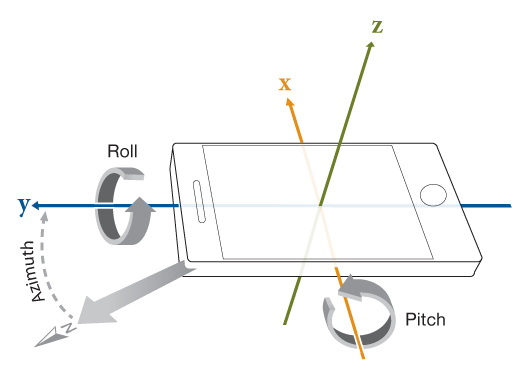
\includegraphics[width=0.85\textwidth]{img/smartphone_axis.png}
\caption{\label{fig:axis-smartphone}Axis orientation in a smartphone}
\end{figure}
%
In order to test this concept, the code presented in \ref{sec:accelerometer-data} that refers to the accelerometer was added to another project that allowed ball movement based on the accelerometer values. It must be noticed that the z acceleration value it's not relevant to the ball movement (from line 59 to 67) since only \textbf{roll} and \textbf{pitch} affect a 2D (bidimensional) object and the smartphone height relative to the ground doesn't, as one should expect by analysing figure \ref{fig:axis-smartphone}.
%
This code in listing \ref{lst:ball_mov} representing subsection \ref{sec:accelerometer-access} will be tested in \ref{sec:accelerometer-using-data-test}.\\
%
\lstinputlisting[language=Java,caption={Code for ball movement based on accelerometer data},label=lst:ball_mov,style=custom-java]{listing/ballMovement.java}
%
%
\subsection{Bluetooth}%
\label{sec:bluetooth-implem}
%
Bluetooth is one of the communication technologies specified in the project analysis (section \ref{ch:analysis}), hence it is important to assure the data flow between the smartphone and the \gls{nvs} on another redundancy communication failure like Wi-Fi. 
%
\subsubsection{Bluetooth Connection Setup}
\label{sec:bluetooth-connection-setup}
Starting from the design and reusing previous Java code made on other course units (based on \cite{btchatsrc}), the Bluetooth setup was implemented on Android Studio and then deployed in a smartphone, the code is depicted in listing \ref{lst:bt-setup}.
%
Note that the forementioned code has \textbf{threads} to simulate parallel computing since the app should be able to send data to the paired device and receive data from it.
%
In lines 10, 11 and 12, are represented the three thread classes used for the Bluetooth connection setup. These classes inherit from the \textbf{Thread class} (\underline{extends Thread} - line 114), considering it must exist \textbf{concurrency} and \textbf{resource sharing} for the application to send and receive data simultaneously. 
%
The \textbf{AcceptThread} (line 10) it's related to the discovery of new connections since it plays an important role in the creation of a \textbf{BluetoothServerSocket} that allows two intended devices to find and accept each other as a part of the initial device inquiry prior to the connection stage. Line 11 represents the \textbf{ConnectThread} responsible for managing the connection between two devices. This thread starts as soon as the two devices accept each other and then proceeds to create a \textbf{RfcommSocket} and connect the devices (pair) when the user clicks on an unpaired device from the list presented. Finally, the \textbf{IOThread} assures the message exchange between devices by accessing the input and output streams of the \textbf{Bluetooth Socket}.
%
As stated earlier, it was necessary to make some includes in the Bluetooth app as well as virtualize some ports in order to interface the \gls{pc} virtual machine with the smartphone, this will be more thoroughly explained in the testing section (\ref{sec:bluetooth-phone-nvs}).
%
Finally, from the smartphone point of view, the protocol purpose was to transmit commands to control the vehicle by sending the phone accelerometers' values and receive its message warnings on screen.\\
%
\lstinputlisting[language=Java,caption={Code for bluetooth connection setup},label=lst:bt-setup,style=custom-java]{listing/btSetup.java}
%
%%% Local Variables:
%%% mode: latex
%%% TeX-master: "../../../dissertation"
%%% End:



%
\subsection{Wi-Fi}%
\label{sec:wifi-implem}
%
Wi-Fi is the second communication technology adopted to guarantee effective control of the rover with the commands from the smartphone.
%
\subsubsection{Wi-Fi Connection Setup}
\label{sec:wifi-implem-connection}
%
The Wi-Fi connection setup code implementation is listed in \ref{lst:wifi-connection-setup}. As one would expect it follows a \textbf{client-server approach} represented in the mentioned listing by the classes \textbf{ServerClass} (line 218) and \textbf{ClientClass} (line 238). Note that both classes inherit from the \textbf{Thread} class since, once again, \textbf{concurrency} is a relevant factor. On one hand, the \textbf{ServerClass} it's responsible for creating a \textbf{ServerSocket} and specify the port that will be used in the connection. This type of protocol usually requires the determination of the IP address and port number that will be utilized. On the other hand, the \textbf{ClientClass} also has to specify the port used but also the forementioned IP. Due to the programming language option chosen in section \ref{sec:smartphone-implem}, one is now limited to use the predetermined IP protocol version preemptively defined (in this case \textbf{IPv6}) what might not be optimal. Both classes use another class that inherits from \textbf{Thread}, the \textbf{WifiConnectionManager} class, to handle the\textbf{ Wi-Fi input and output streams} of the \textbf{server and client sockets}, if the device is host or client, respectively. With this \textbf{WifiConnectionManager} class, one can manage the message exchange between the devices and assure its simultaneity.\\
%
\lstinputlisting[language=Java,caption={Code for Wi-fi connection setup},label=lst:wifi-connection-setup,style=custom-java]{listing/wifiConnectionImplem.java}
%
\subsubsection{Wi-Fi Video Feed}
\label{sec:wifi-implem-video}
%
One important user feature defined in the design of the smartphone application in section \ref{sec:smartphone-design} was the capability of watching the \gls{rvvs}' live camera feed within the app. The applied solution is based on the \textbf{Youtube Android Player \gls{api}} \cite{yt_api} as it enables a more \textbf{reliable video stream} whilst ensuring \textbf{project off-load}. Resorting to the latter, one can also tackle the fullscreen video display which was a big concern in terms of user-friendliness. Nevertheless, one can still claim that a framewise transmission approach via Wi-Fi is even more fail-safe and secure since one doesn't need to rely on an external entity for video communication.
Despite this, the framewise approach was discarded to ensure deadline meeting, hence its implementation required some prior subject experience or further research. The implementation of the abovementioned feature is depicted in listing \ref{lst:video-view}.\\
%
\lstinputlisting[language=Java,caption={Code for video feed view within the application},label=lst:video-view,style=custom-java]{listing/videoFeed.java}
%

%
\subsection{User Interface}%
\label{sec:ui-implementation}
%
The UI implementation consists of various \textbf{XML files complemented with java code}. Consequently, one can consider the UI features and present images related to those rather than simply overload the document with XML code. Firstly, as one enters the app, an initial screen is presented (figure \ref{fig:app-overview} - \textbf{1}), in this screen the app checks for if the phone supports the Bluetooth services necessary to run the application and requests user permission to enable Bluetooth (figure \ref{fig:app-overview} - \textbf{2}). The second and main screen of the app is composed of a navigation drawer (figure \ref{fig:app-overview} - \textbf{4}) and a screen with two buttons for initiating the video stream (figure \ref{fig:app-overview} - \textbf{3}). The navigation drawer is the place where the user can perform all the communication-related actions like enabling Wifi or setting up a Wi-fi or Bluetooth connection. The aforesaid main screen also as has a status indicator. As one enters the rover control screen (figure \ref{fig:app-overview} - \textbf{11}) the orientation is automatically changed to the one (preemptively defined) that allows the correct initial position for the car control. In this screen, one can see the RVVS' live transmission and the speed and wheel tilt percentages sent to the same module. The video allows the fullscreen display (figure \ref{fig:app-overview} - \textbf{9,10,12}), still showing the latter percentages as a periodic pop-up (figure \ref{fig:app-overview} - \textbf{9}). Note that one tried to achieve a balance between app functionality while also creating a user-friendly environment.
%
\begin{figure}[!ht]
\centering
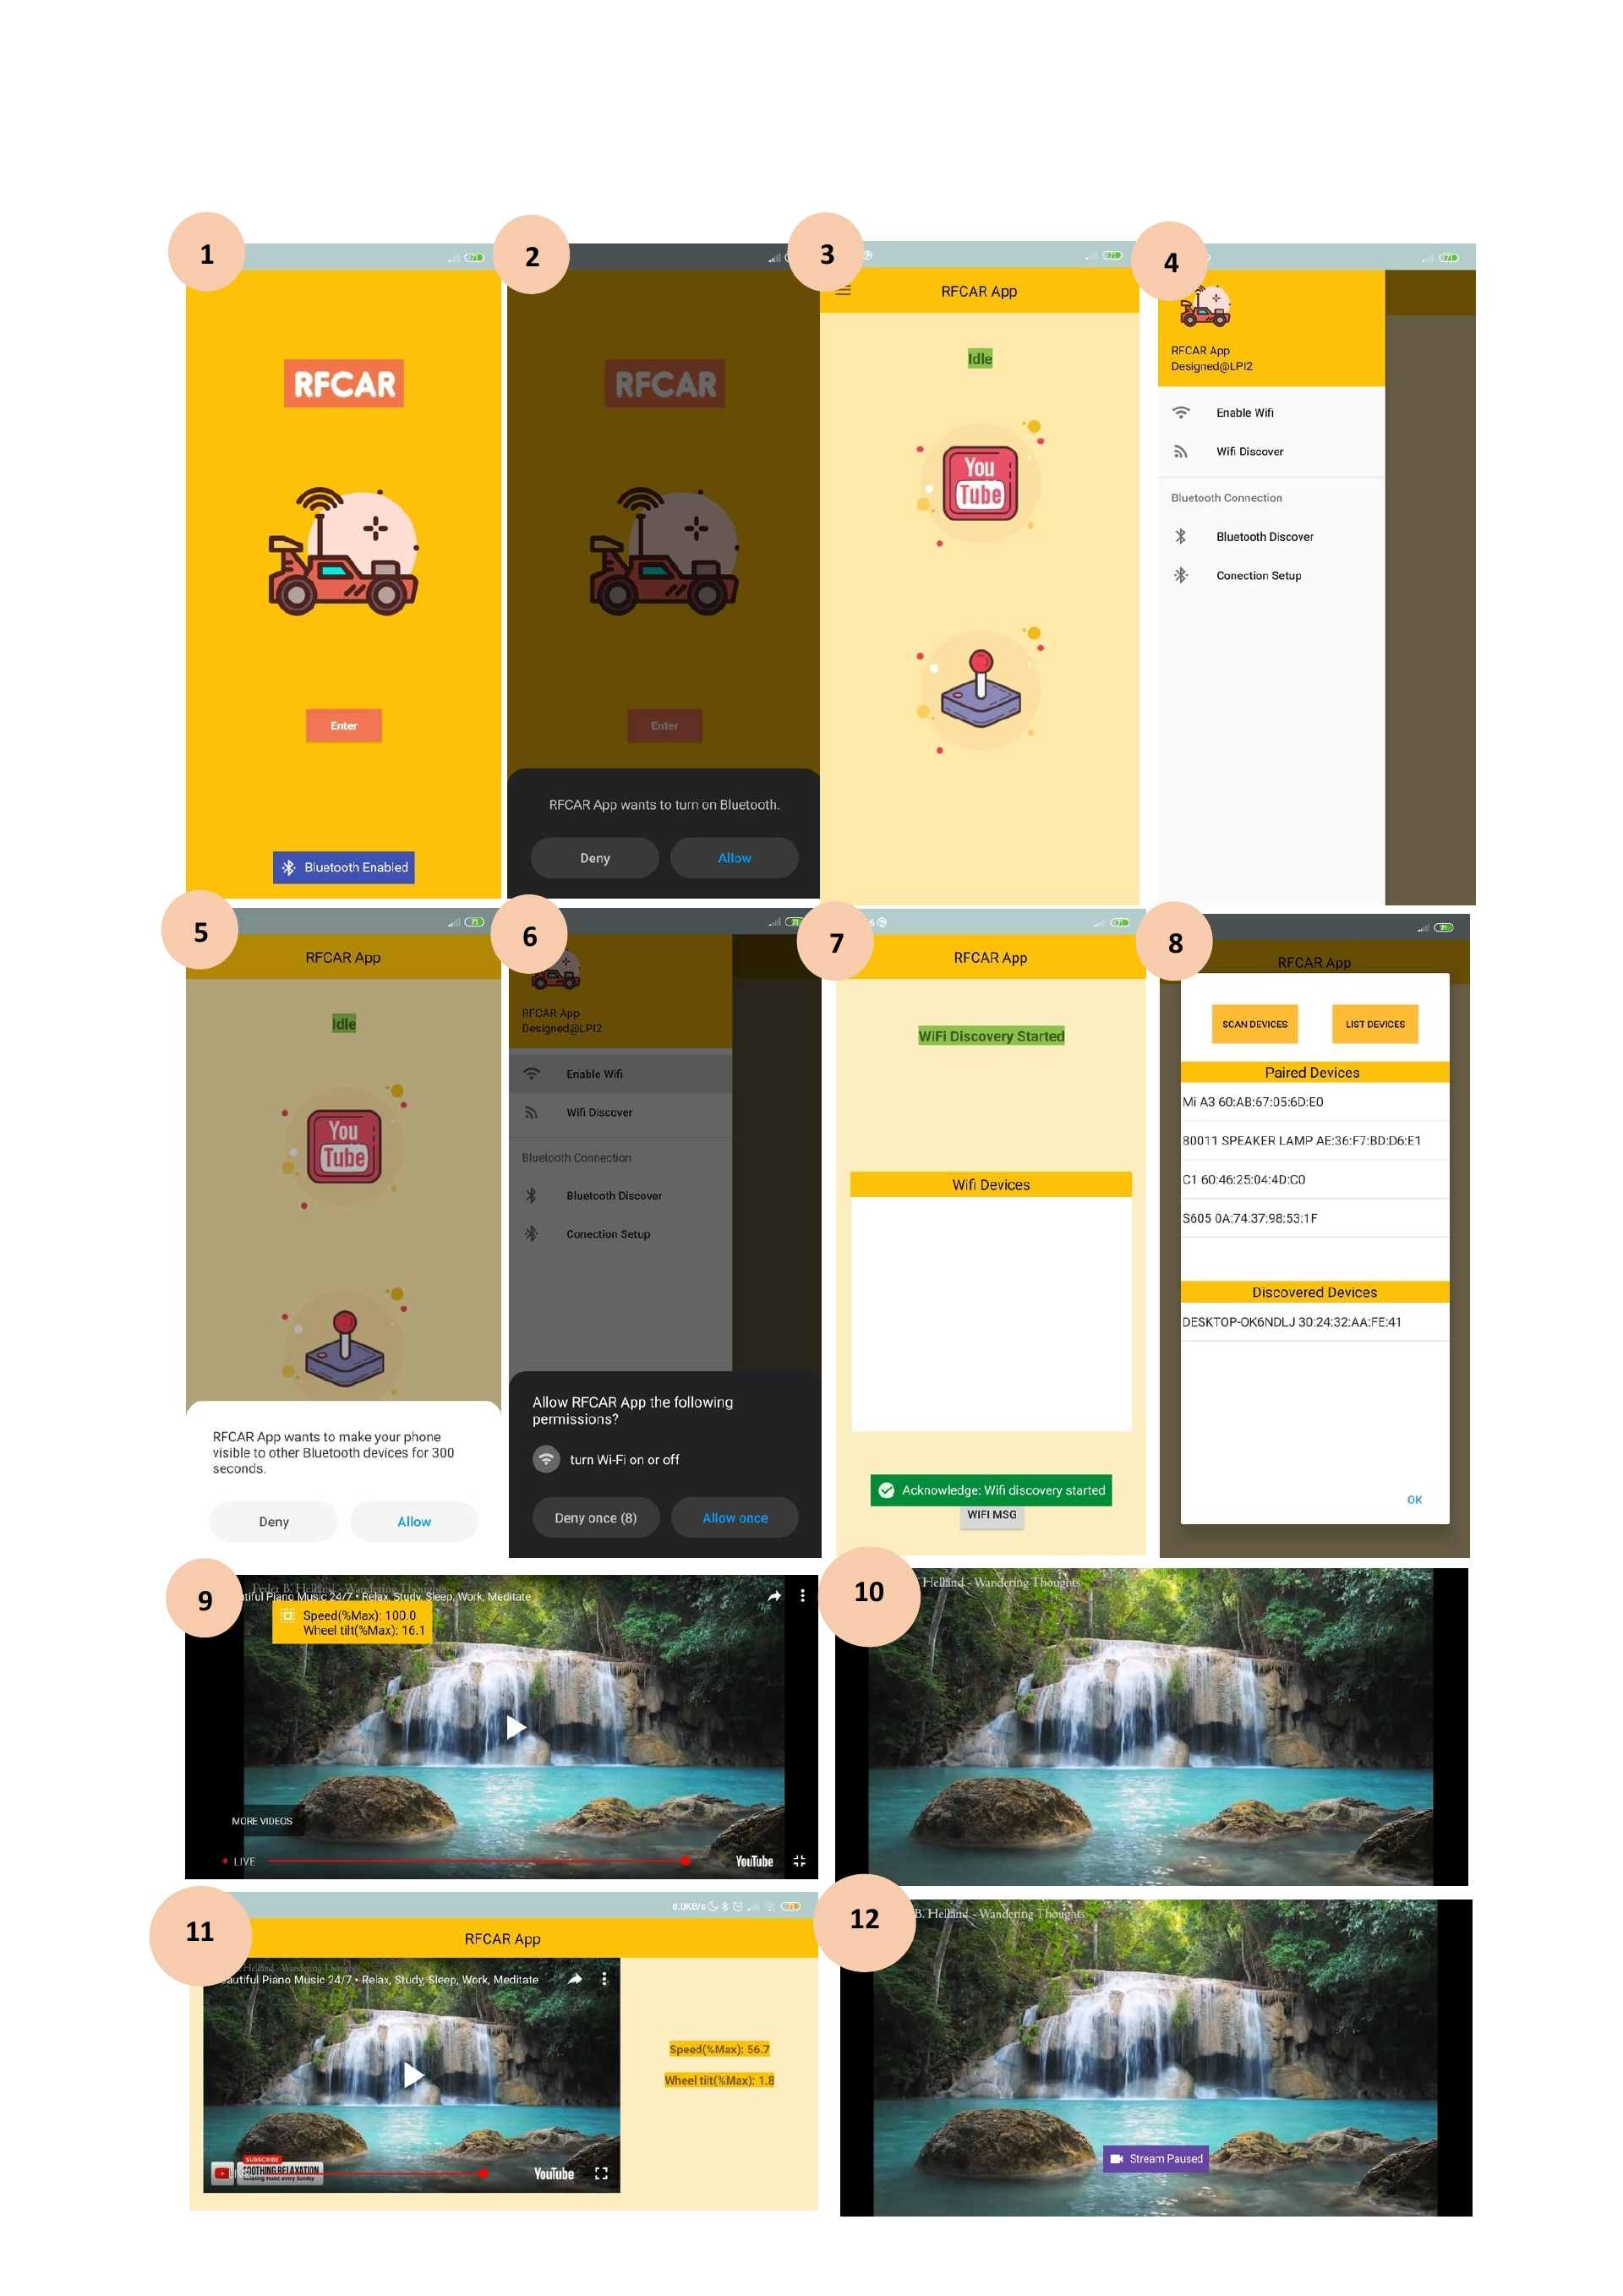
\includegraphics[width=0.75\textwidth]{img/general-app-overview.jpg}
\caption{\label{fig:app-overview}General App Overview}
\end{figure}
%
%